\section{Appendix}
\subsection{Simple Static Extension}
\subsubsection{OLS Solution}
In case the population covariance matrix is observable, the OLS-coefficients can be directly derived from it: $\left( w_1^{OLS}, w_2^{OLS} \right) = \boldsymbol{\Sigma_2}^{-1} \boldsymbol{\sigma_{12}}  $
\subsubsection{SC Solution}
The restricted solution is can directly be derived from the covariance matrix. The first index in the square brackets indicates the row, the second the column position. 
\begin{equation*}
	\begin{split}
		w_1^{SC} & = \left( \boldsymbol{\sigma_{12}}^\prime[1] - \boldsymbol{\sigma_{12}}^\prime[2] - \boldsymbol{\Sigma_2}[2,1] + \boldsymbol{\Sigma_2}[1,1] \right) / \left( \boldsymbol{\Sigma_2}[1,1] + \boldsymbol{\Sigma_2}[2,2] - 2 * \boldsymbol{\Sigma_2}[1,2] \right) \\
		& = (0.1-0.4-0.5+1)/(1+1-2*0.5) = 0.2 
	\end{split} 
\end{equation*}
\begin{equation*}
	\begin{split}
		w_2^{SC} & = \left( \boldsymbol{\sigma_{12}}^\prime[2] - \boldsymbol{\sigma_{12}}^\prime[1] - \boldsymbol{\Sigma_2}[1,2] + \boldsymbol{\Sigma_2}[2,2] \right) / \left( \boldsymbol{\Sigma_2}[2,2] + \boldsymbol{\Sigma_2}[1,1] - 2 * \boldsymbol{\Sigma_2}[2,1] \right) \\
		& = (0.4-0.1-0.5+1)/(1+1-2*0.5) = 0.8
	\end{split}
\end{equation*}
\subsubsection{Variances}
The variances are derived from the weights and the covariance matrix:
\begin{equation*}
	\begin{split}
		var(Y_0 - w_1 Y_1 - w_2 Y_2) = &\text{ }var(Y_0) + w_1^2 \cdot var(Y_1) + w_2^2 \cdot var(Y_2)\text{ }- \\
		& 2 \cdot w_1 \cdot cov(Y_0, Y_1) - 2 \cdot w_2 \cdot cov(Y_0, Y_2)\text{ }+ \\
		&2 \cdot w_1 w_2 \cdot cov(Y_1, Y_2) 
	\end{split}
\end{equation*}

\newpage
\subsection{General Static Extension}
\subsubsection{REGSC: The limit for $\lambda_1\to \infty$ and $\lambda_2 \to \infty$}

For $\lambda_1\to \infty$ and $\lambda_2\to \infty$ the objective function reduce to
\begin{align*}
	Q(\lambda_1,\lambda2) &= \lambda_1 w'w + \lambda_2 (1-\mathbf{1}'w)^2
\end{align*}
The derivative is obtained as
\begin{align*}
	\frac{ \partial Q(\lambda_1,\lambda_2) }{ \partial w} &= 2 \lambda_1 w + 2 \lambda_2 (\mathbf{1}-\mathbf{1} \mathbf{1}'w)
\end{align*}
By setting the derivative to zero and multiplying with $\mathbf{1}$ we obtain:
\begin{align*}
	\lambda_1 \mathbf{1}'w + \lambda_2 (n- \mathbf{1}'w) = 0
\end{align*}
where $\mathbf{1}'w =\sum w_i$. Solving for $ \mathbf{1}'w $ we obtain
\begin{align*}
	\mathbf{1}'w  &= \frac{ 1}{ 1 +\lambda_1/\lambda_2 }
\end{align*}
and due to the symmetry of the objective function with respect to the elements of the weight vector we have
\begin{align*}
	w_i &= 1/(n+n\lambda_1/\lambda_2)
\end{align*}


\subsection{Simulation Study}
\subsubsection{Static Simulation results}
\label{Static simulation}
\newpage
\begin{table}[H]
	\centering
	\noindent
	\caption{Simulation Results of the Static Factor Model with \textbf{J = 5} Donors.}
	\scalebox{1}{
		\begin{tabular}{c c | C{2.48cm} | C{2.48cm} | C{2.48cm} | C{2.48cm} | C{2.48cm} }
			\toprule[1.5pt]
			\multicolumn{1}{c}{$\boldsymbol{T_{pre}}$} & \multicolumn{1}{c}{$\boldsymbol{T_{post}}$}& \multicolumn{1}{c}{\textbf{FACTOR}} & \multicolumn{1}{c}{\textbf{SC}} & \multicolumn{1}{c}{\textbf{REGSC}}& \multicolumn{1}{c}{\textbf{NET}}& \multicolumn{1}{c}{\textbf{OLS}}\\
			\cmidrule(lr){1-7}
			& & RMSE&RMSE&RMSE&RMSE&RMSE\\
			& & (BIAS)&(BIAS)&(BIAS)&(BIAS)&(BIAS)\\
			& & [MZ-RATES] & [MZ-RATES] & [MZ-RATES] &[MZ-RATES] &[MZ-RATES]\\
			& & \{VARIANCE\} & \{VARIANCE\}& \{VARIANCE\}&\{VARIANCE\} &\{VARIANCE\}\\
			\cmidrule(lr){1-7}
			20&30&1.2497&1.4455&1.3064&1.3086&1.3814\\
			&&(-0.0045)&(-0.0086)&(-0.0144)&(-0.0073)&(-0.0098)\\
			&&[0.7250]&[0.4210]&[0.6240]&[0.6691]&[0.5140]\\
			&&\{0.6523\}&\{1.1179\}&\{0.6898\}&\{0.6581\}&\{1.1678\}\\
			&20&1.2509&1.4575&1.3054&1.3048&1.3661\\
			&&(0.0137)&(0.0331)&(0.0063)&(0.0085)&(0.0114)\\
			&&[0.8240]&[0.5360]&[0.7460]&[0.7516]&[0.6650]\\
			&&\{0.6143\}&\{1.0690\}&\{0.6619\}&\{0.6137\}&\{1.1028\}\\
			&10&1.2344&1.4283&1.2847&1.2804&1.3520\\
			&&(-0.0092)&(-0.0120)&(-0.0075)&(-0.0098)&(-0.0126)\\
			&&[0.8940]&[0.7380]&[0.8540]&[0.8723]&[0.8060]\\
			&&\{0.6137\}&\{1.0366\}&\{0.6505\}&\{0.6086\}&\{1.0948\}\\
			\cmidrule(lr){1-7}
			% next specification
			50&30&1.1831&1.4185&1.2131&1.2045&1.2190\\
			&&(0.0147)&(-0.0223)&(0.0137)&(0.0117)&(0.0106)\\
			&&[0.8510]&[0.4600]&[0.8210]&[0.8388]&[0.8250]\\
			&&\{0.6459\}&\{1.0600\}&\{0.6440\}&\{0.5834\}&\{0.7974\}\\
			&20&1.1740&1.4160&1.2044&1.1948&1.2105\\
			&&(-0.0195)&(-0.0106)&(-0.0204)&(-0.0191)&(-0.0166)\\
			&&[0.9030]&[0.5630]&[0.8650]&[0.8810]&[0.8750]\\
			&&\{0.6426\}&\{1.0680\}&\{0.6311\}&\{0.5752\}&\{0.7879\}\\
			&10&1.1635&1.4033&1.1940&1.1845&1.2009\\
			&&(-0.0081)&(-0.0211)&(-0.0115)&(-0.0081)&(-0.0074)\\
			&&[0.9300]&[0.7340]&[0.9170]&[0.9260]&[0.9120]\\
			&&\{0.5963\}&\{1.0002\}&\{0.5850\}&\{0.5407\}&\{0.7415\}\\
			\cmidrule(lr){1-7}
			% next specification
			100&30&1.1645&1.3955&1.1811&1.1733&1.1799\\
			&&(0.0047)&(0.0381)&(0.0053)&(0.0048)&(0.0052)\\
			&&[0.8920]&[0.4950]&[0.8700]&[0.8930]&[0.8870]\\
			&&\{0.6494\}&\{1.0668\}&\{0.6405\}&\{0.5931\}&\{0.7238\}\\
			&20&1.1576&1.3796&1.1756&1.1691&1.1755\\
			&&(0.0026)&(-0.0384)&(0.0040)&(0.0021)&(0.0012)\\
			&&[0.9220]&[0.6080]&[0.9100]&[0.9120]&[0.9100]\\
			&&\{0.6389\}&\{1.0337\}&\{0.6226\}&\{0.5871\}&\{0.7090\}\\
			&10&1.1518&1.3907&1.1682&1.1643&1.1697\\
			&&(0.0108)&(0.0592)&(0.0156)&(0.0146)&(0.0135)\\
			&&[0.9440]&[0.7570]&[0.9370]&[0.9400]&[0.9330]\\
			&&\{0.5971\}&\{0.9826\}&\{0.5740\}&\{0.5432\}&\{0.6623\}\\
			\bottomrule[1.5pt]
	\end{tabular}}
	\label{table:table S.1}
\end{table}

\newpage
\begin{table}[H]
	\centering
	\noindent
	\caption{Simulation Results of the Static Factor Model with \textbf{J = 10} Donors.}
	\scalebox{1}{
		\begin{tabular}{c c | C{2.48cm} | C{2.48cm} | C{2.48cm} | C{2.48cm} | C{2.48cm} }
			\toprule[1.5pt]
			\multicolumn{1}{c}{$\boldsymbol{T_{pre}}$} & \multicolumn{1}{c}{$\boldsymbol{T_{post}}$}& \multicolumn{1}{c}{\textbf{FACTOR}} & \multicolumn{1}{c}{\textbf{SC}} & \multicolumn{1}{c}{\textbf{REGSC}}& \multicolumn{1}{c}{\textbf{NET}}& \multicolumn{1}{c}{\textbf{OLS}}\\
			\cmidrule(lr){1-7}
			& & RMSE&RMSE&RMSE&RMSE&RMSE\\
			& & (BIAS)&(BIAS)&(BIAS)&(BIAS)&(BIAS)\\
			& & [MZ-RATES] & [MZ-RATES] & [MZ-RATES] &[MZ-RATES] &[MZ-RATES]\\
			& & \{VARIANCE\} & \{VARIANCE\}& \{VARIANCE\}&\{VARIANCE\} &\{VARIANCE\}\\
			\cmidrule(lr){1-7}
			20&30&1.1575&1.2944&1.2229&1.2521&1.6286\\
			&&(-0.0071)&(0.0002)&(-0.0047)&(-0.0093)&(0.0018)\\
			&&[0.7090]&[0.5720]&[0.6590]&[0.6416]&[0.1790]\\
			&&\{0.7830\}&\{1.0468\}&\{0.7805\}&\{0.7714\}&\{2.3061\}\\
			&20&1.1611&1.2759&1.2336&1.2591&1.6075\\
			&&(0.0060)&(0.0197)&(0.0071)&(0.0036)&(0.0045)\\
			&&[0.8220]&[0.6920]&[0.7590]&[0.7495]&[0.3520]\\
			&&\{0.7459\}&\{1.0523\}&\{0.7777\}&\{0.7613\}&\{2.1785\}\\
			&10&1.1675&1.2963&1.2318&1.2659&1.6276\\
			&&(0.0040)&(0.0127)&(0.0004)&(0.0006)&(0.0181)\\
			&&[0.8840]&[0.8050]&[0.8550]&[0.8513]&[0.6020]\\
			&&\{0.6883\}&\{0.9859\}&\{0.7180\}&\{0.6984\}&\{2.0705\}\\
			\cmidrule(lr){1-7}
			% next specification
			50&30&1.1048&1.2511&1.1444&1.1524&1.2140\\
			&&(0.0049)&(0.0020)&(0.0079)&(0.0065)&(0.0087)\\
			&&[0.8640]&[0.6680]&[0.8240]&[0.8310]&[0.7420]\\
			&&\{0.7755\}&\{1.0148\}&\{0.7207\}&\{0.6795\}&\{1.1008\}\\
			&20&1.0985&1.2416&1.1327&1.1417&1.2022\\
			&&(0.0047)&(0.0037)&(0.0029)&(0.0042)&(0.0028)\\
			&&[0.8870]&[0.7270]&[0.8750]&[0.8750]&[0.8190]\\
			&&\{0.7744\}&\{0.9962\}&\{0.7333\}&\{0.6573\}&\{1.0658\}\\
			&10&1.0838&1.2171&1.1183&1.1270&1.1857\\
			&&(0.0001)&(0.0033)&(-0.0039)&(-0.0034)&(-0.0049)\\
			&&[0.9310]&[0.8560]&[0.9370]&[0.9290]&[0.9100]\\
			&&\{0.7704\}&\{0.9989\}&\{0.7199\}&\{0.6649\}&\{1.0604\}\\
			\cmidrule(lr){1-7}
			% next specification
			100&30&1.0920&1.2323&1.1141&1.1171&1.1405\\
			&&(0.0040)&(0.0119)&(0.0050)&(0.0039)&(0.0025)\\
			&&[0.9070]&[0.6930]&[0.9040]&[0.9080]&[0.8780]\\
			&&\{0.8025\}&\{1.0112\}&\{0.7620\}&\{0.6968\}&\{0.9363\}\\
			&20&1.0842&1.2232&1.1073&1.1088&1.1333\\
			&&(-0.0057)&(-0.0031)&(-0.0049)&(-0.0064)&(-0.0081)\\
			&&[0.9360]&[0.7680]&[0.9240]&[0.9280]&[0.9150]\\
			&&\{0.7858\}&\{1.0095\}&\{0.7427\}&\{0.6902\}&\{0.9314\}\\
			&10&1.0742&1.2059&1.0919&1.0986&1.1186\\
			&&(0.0080)&(-0.0206)&(0.0021)&(0.0016)&(0.0006)\\
			&&[0.9400]&[0.8660]&[0.9340]&[0.9470]&[0.9430]\\
			&&\{0.7377\}&\{0.9476\}&\{0.6925\}&\{0.6526\}&\{0.8653\}\\
			\bottomrule[1.5pt]
	\end{tabular}}
	\label{table:table S.2}
\end{table}

\newpage
\begin{table}[H]
	\centering
	\noindent
	\caption{Simulation Results of the Static Factor Model with \textbf{J = 15} Donors.}
	\scalebox{1}{
		\begin{tabular}{c c | C{2.48cm} | C{2.48cm} | C{2.48cm} | C{2.48cm} | C{2.48cm} }
			\toprule[1.5pt]
			\multicolumn{1}{c}{$\boldsymbol{T_{pre}}$} & \multicolumn{1}{c}{$\boldsymbol{T_{post}}$}& \multicolumn{1}{c}{\textbf{FACTOR}} & \multicolumn{1}{c}{\textbf{SC}} & \multicolumn{1}{c}{\textbf{REGSC}}& \multicolumn{1}{c}{\textbf{NET}}& \multicolumn{1}{c}{\textbf{OLS}}\\
			\cmidrule(lr){1-7}
			& & RMSE&RMSE&RMSE&RMSE&RMSE\\
			& & (BIAS)&(BIAS)&(BIAS)&(BIAS)&(BIAS)\\
			& & [MZ-RATES] & [MZ-RATES] & [MZ-RATES] &[MZ-RATES] &[MZ-RATES]\\
			& & \{VARIANCE\} & \{VARIANCE\}& \{VARIANCE\}&\{VARIANCE\} &\{VARIANCE\}\\
			\cmidrule(lr){1-7}
			20&30&1.1398&1.2604&1.2276&1.2533&2.4777\\
			&&(0.0243)&(0.0374)&(0.0244)&(0.0197)&(0.0312)\\
			&&[0.7340]&[0.6240]&[0.6450]&[0.6408]&[0.0320]\\
			&&\{0.7617\}&\{1.0341\}&\{0.8403\}&\{0.7997\}&\{6.3624\}\\
			&20&1.1287&1.2417&1.2149&1.2432&2.4716\\
			&&(0.0042)&(0.0258)&(0.0129)&(0.0165)&(-0.0097)\\
			&&[0.8200]&[0.7250]&[0.7460]&[0.7386]&[0.0690]\\
			&&\{0.7481\}&\{0.9966\}&\{0.8261\}&\{0.7667\}&\{6.3819\}\\
			&10&1.1112&1.2309&1.1973&1.2167&2.4393\\
			&&(0.0206)&(-0.0240)&(0.0224)&(0.0247)&(0.0245)\\
			&&[0.9030]&[0.8540]&[0.8640]&[0.8660]&[0.2450]\\
			&&\{0.7130\}&\{0.9484\}&\{0.7702\}&\{0.7234\}&\{6.0769\}\\
			\cmidrule(lr){1-7}
			% next specification
			50&30&1.0818&1.1935&1.1198&1.1356&1.2747\\
			&&(-0.0032)&(0.0006)&(-0.0019)&(-0.0019)&(-0.0040)\\
			&&[0.8580]&[0.7490]&[0.8230]&[0.8070]&[0.5980]\\
			&&\{0.8282\}&\{1.0035\}&\{0.7778\}&\{0.7102\}&\{1.3448\}\\
			&20&1.0879&1.1975&1.1307&1.1470&1.2892\\
			&&(-0.0133)&(-0.0183)&(-0.0205)&(-0.0188)&(-0.0210)\\
			&&[0.8950]&[0.8060]&[0.8710]&[0.8760]&[0.6930]\\
			&&\{0.7705\}&\{0.9465\}&\{0.7340\}&\{0.6722\}&\{1.2960\}\\
			&10&1.0522&1.1754&1.0896&1.1004&1.2281\\
			&&(-0.0132)&(-0.0098)&(-0.0130)&(-0.0122)&(-0.0011)\\
			&&[0.9240]&[0.8650]&[0.9170]&[0.9210]&[0.8460]\\
			&&\{0.7913\}&\{0.9519\}&\{0.7423\}&\{0.6776\}&\{1.2605\}\\
			\cmidrule(lr){1-7}
			% next specification
			100&30&1.0678&1.1818&1.0890&1.0974&1.1415\\
			&&(0.0007)&(-0.0212)&(0.0007)&(-0.0004)&(-0.0034)\\
			&&[0.8950]&[0.7310]&[0.8900]&[0.8730]&[0.8310]\\
			&&\{0.8395\}&\{0.9981\}&\{0.7767\}&\{0.7073\}&\{1.0481\}\\
			&20&1.0667&1.1809&1.0886&1.0947&1.1468\\
			&&(0.0048)&(-0.0018)&(0.0073)&(0.0064)&(0.0066)\\
			&&[0.9290]&[0.8040]&[0.9230]&[0.9180]&[0.8800]\\
			&&\{0.8321\}&\{0.9770\}&\{0.7671\}&\{0.6998\}&\{1.0384\}\\
			&10&1.0411&1.1459&1.0654&1.0717&1.1200\\
			&&(-0.0059)&(-0.0049)&(-0.0045)&(-0.0057)&(-0.0056)\\
			&&[0.9310]&[0.8740]&[0.9290]&[0.9290]&[0.9120]\\
			&&\{0.7897\}&\{0.9161\}&\{0.7422\}&\{0.6802\}&\{0.9948\}\\
			\bottomrule[1.5pt]
	\end{tabular}}
	\label{table:table S.3}
\end{table}

\newpage
\begin{table}[H]
	\centering
	\noindent
	\caption{Simulation Results of the Static Factor Model with \textbf{J = 20} Donors.}
	\scalebox{1}{
		\begin{tabular}{c c | C{2.48cm} | C{2.48cm} | C{2.48cm} | C{2.48cm} | C{2.48cm} }
			\toprule[1.5pt]
			\multicolumn{1}{c}{$\boldsymbol{T_{pre}}$} & \multicolumn{1}{c}{$\boldsymbol{T_{post}}$}& \multicolumn{1}{c}{\textbf{FACTOR}} & \multicolumn{1}{c}{\textbf{SC}} & \multicolumn{1}{c}{\textbf{REGSC}}& \multicolumn{1}{c}{\textbf{NET}}& \multicolumn{1}{c}{\textbf{OLS}}\\
			\cmidrule(lr){1-7}
			& & RMSE&RMSE&RMSE&RMSE&RMSE\\
			& & (BIAS)&(BIAS)&(BIAS)&(BIAS)&(BIAS)\\
			& & [MZ-RATES] & [MZ-RATES] & [MZ-RATES] &[MZ-RATES] &[MZ-RATES]\\
			& & \{VARIANCE\} & \{VARIANCE\}& \{VARIANCE\}&\{VARIANCE\} &\{VARIANCE\}\\
			\cmidrule(lr){1-7}
			20&30&1.1228&1.2229&1.2040&1.2331&NA\\
			&&(0.0074)&(-0.0229)&(0.0044)&(-0.0010)&(NA)\\
			&&[0.7090]&[0.6550]&[0.6410]&[0.6079]&[NA]\\
			&&\{0.8229\}&\{1.0024\}&\{0.8544\}&\{0.8238\}&\{NA\}\\
			&20&1.1230&1.2276&1.2093&1.2385&NA\\
			&&(0.0009)&(-0.0067)&(-0.0008)&(-0.0041)&(NA)\\
			&&[0.8030]&[0.7520]&[0.7250]&[0.7144]&[NA]\\
			&&\{0.7731\}&\{0.9833\}&\{0.8563\}&\{0.8207\}&\{NA\}\\
			&10&1.0939&1.1927&1.1749&1.2036&NA\\
			&&(0.0023)&(-0.0226)&(0.0033)&(0.0031)&(NA)\\
			&&[0.8860]&[0.8730]&[0.8480]&[0.8357]&[NA]\\
			&&\{0.7695\}&\{0.9365\}&\{0.8217\}&\{0.7697\}&\{NA\}\\
			\cmidrule(lr){1-7}
			% next specification
			50&30&1.0662&1.1629&1.1007&1.1180&1.3564\\
			&&(-0.0121)&(-0.0148)&(-0.0141)&(-0.0182)&(-0.0184)\\
			&&[0.8640]&[0.7290]&[0.8330]&[0.8230]&[0.4080]\\
			&&\{0.8580\}&\{0.9743\}&\{0.7912\}&\{0.7118\}&\{1.6096\}\\
			&20&1.0702&1.1693&1.1085&1.1205&1.3538\\
			&&(0.0004)&(0.0055)&(-0.0004)&(0.0008)&(-0.0073)\\
			&&[0.8810]&[0.8070]&[0.8710]&[0.8690]&[0.5880]\\
			&&\{0.8213\}&\{0.9484\}&\{0.7632\}&\{0.7049\}&\{1.5678\}\\
			&10&1.0566&1.1627&1.0907&1.1086&1.3371\\
			&&(0.0204)&(0.0143)&(0.0234)&(0.0242)&(0.0204)\\
			&&[0.9280]&[0.8950]&[0.9230]&[0.9230]&[0.8060]\\
			&&\{0.7780\}&\{0.9080\}&\{0.7208\}&\{0.6595\}&\{1.4765\}\\
			\cmidrule(lr){1-7}
			% next specification
			100&30&1.0512&1.1442&1.0735&1.0856&1.1639\\
			&&(-0.0083)&(0.0027)&(-0.0072)&(-0.0073)&(-0.0066)\\
			&&[0.9040]&[0.7800]&[0.8820]&[0.8890]&[0.7880]\\
			&&\{0.8556\}&\{0.9709\}&\{0.7933\}&\{0.7236\}&\{1.1355\}\\
			&20&1.0438&1.1434&1.0652&1.0763&1.1584\\
			&&(-0.0035)&(0.0063)&(-0.0009)&(-0.0030)&(-0.0035)\\
			&&[0.9230]&[0.8380]&[0.9260]&[0.9200]&[0.8400]\\
			&&\{0.8657\}&\{0.9643\}&\{0.7987\}&\{0.7379\}&\{1.1555\}\\
			&10&1.0381&1.1236&1.0615&1.0729&1.1502\\
			&&(-0.0014)&(-0.0054)&(0.0005)&(-0.0024)&(-0.0035)\\
			&&[0.9510]&[0.9110]&[0.9460]&[0.9380]&[0.9160]\\
			&&\{0.8044\}&\{0.8937\}&\{0.7387\}&\{0.6780\}&\{1.0692\}\\
			\bottomrule[1.5pt]
	\end{tabular}}
	\label{table:table S.4}
\end{table}

\newpage
\begin{table}[H]
	\centering
	\noindent
	\caption{Simulation Results of the Static Factor Model with \textbf{J = 25} Donors.}
	\scalebox{1}{
		\begin{tabular}{c c | C{2.48cm} | C{2.48cm} | C{2.48cm} | C{2.48cm} | C{2.48cm} }
			\toprule[1.5pt]
			\multicolumn{1}{c}{$\boldsymbol{T_{pre}}$} & \multicolumn{1}{c}{$\boldsymbol{T_{post}}$}& \multicolumn{1}{c}{\textbf{FACTOR}} & \multicolumn{1}{c}{\textbf{SC}} & \multicolumn{1}{c}{\textbf{REGSC}}& \multicolumn{1}{c}{\textbf{NET}}& \multicolumn{1}{c}{\textbf{OLS}}\\
			\cmidrule(lr){1-7}
			& & RMSE&RMSE&RMSE&RMSE&RMSE\\
			& & (BIAS)&(BIAS)&(BIAS)&(BIAS)&(BIAS)\\
			& & [MZ-RATES] & [MZ-RATES] & [MZ-RATES] &[MZ-RATES] &[MZ-RATES]\\
			& & \{VARIANCE\} & \{VARIANCE\}& \{VARIANCE\}&\{VARIANCE\} &\{VARIANCE\}\\
			\cmidrule(lr){1-7}
			20&30&1.1154&NA&1.2097&1.2225&NA\\
			&&(0.0019)&(NA)&(-0.0002)&(-0.0036)&(NA)\\
			&&[0.6980]&[NA]&[0.6280]&[0.6440]&[NA]\\
			&&\{0.8012\}&\{NA\}&\{0.8593\}&\{0.7918\}&\{NA\}\\
			&20&1.1038&NA&1.2001&1.2240&NA\\
			&&(0.0081)&(NA)&(0.0127)&(0.0125)&(NA)\\
			&&[0.8150]&[NA]&[0.7410]&[0.7310]&[NA]\\
			&&\{0.7882\}&\{NA\}&\{0.8314\}&\{0.7967\}&\{NA\}\\
			&10&1.1051&NA&1.1829&1.2061&NA\\
			&&(0.0056)&(NA)&(-0.0046)&(-0.0038)&(NA)\\
			&&[0.8830]&[NA]&[0.8590]&[0.8513]&[NA]\\
			&&\{0.7503\}&\{NA\}&\{0.7897\}&\{0.7621\}&\{NA\}\\
			\cmidrule(lr){1-7}
			% next specification
			50&30&1.0657&1.1525&1.1039&1.1198&1.4937\\
			&&(0.0104)&(-0.0014)&(0.0121)&(0.0119)&(0.0138)\\
			&&[0.8510]&[0.7880]&[0.8390]&[0.8270]&[0.2260]\\
			&&\{0.8576\}&\{0.9696\}&\{0.8090\}&\{0.7223\}&\{2.0239\}\\
			&20&1.0541&1.1514&1.0905&1.1090&1.4816\\
			&&(0.0175)&(0.0171)&(0.0202)&(0.0204)&(0.0229)\\
			&&[0.9000]&[0.8460]&[0.8840]&[0.8720]&[0.3860]\\
			&&\{0.8634\}&\{0.9776\}&\{0.8007\}&\{0.7497\}&\{2.0191\}\\
			&10&1.0513&1.1507&1.0911&1.1025&1.4816\\
			&&(-0.0003)&(0.0100)&(-0.0041)&(-0.0056)&(-0.0103)\\
			&&[0.9250]&[0.8930]&[0.9180]&[0.9260]&[0.6880]\\
			&&\{0.8091\}&\{0.9253\}&\{0.7763\}&\{0.7072\}&\{1.9764\}\\
			\cmidrule(lr){1-7}
			% next specification
			100&30&1.0377&1.1262&1.0607&1.0719&1.1913\\
			&&(-0.0036)&(0.0009)&(-0.0028)&(-0.0026)&(0.0002)\\
			&&[0.9190]&[0.8120]&[0.9070]&[0.9000]&[0.7200]\\
			&&\{0.8703\}&\{0.9562\}&\{0.7995\}&\{0.7252\}&\{1.2385\}\\
			&20&1.0431&1.1258&1.0656&1.0778&1.1897\\
			&&(-0.0088)&(-0.0108)&(-0.0075)&(-0.0084)&(-0.0028)\\
			&&[0.9220]&[0.8450]&[0.9180]&[0.9110]&[0.8160]\\
			&&\{0.8747\}&\{0.9594\}&\{0.8108\}&\{0.7317\}&\{1.2371\}\\
			&10&1.0240&1.1119&1.0478&1.0588&1.1803\\
			&&(-0.0011)&(0.0133)&(0.0015)&(0.0023)&(0.0046)\\
			&&[0.9330]&[0.9050]&[0.9250]&[0.9240]&[0.8930]\\
			&&\{0.8335\}&\{0.9086\}&\{0.7689\}&\{0.6957\}&\{1.1779\}\\
			\bottomrule[1.5pt]
	\end{tabular}}
	\label{table:table S.5}
\end{table}

\newpage
\begin{table}[H]
	\centering
	\noindent
	\caption{Simulation Results of the Static Factor Model with \textbf{J = 30} Donors.}
	\scalebox{1}{
		\begin{tabular}{c c | C{2.48cm} | C{2.48cm} | C{2.48cm} | C{2.48cm} | C{2.48cm} }
			\toprule[1.5pt]
			\multicolumn{1}{c}{$\boldsymbol{T_{pre}}$} & \multicolumn{1}{c}{$\boldsymbol{T_{post}}$}& \multicolumn{1}{c}{\textbf{FACTOR}} & \multicolumn{1}{c}{\textbf{SC}} & \multicolumn{1}{c}{\textbf{REGSC}}& \multicolumn{1}{c}{\textbf{NET}}& \multicolumn{1}{c}{\textbf{OLS}}\\
			\cmidrule(lr){1-7}
			& & RMSE&RMSE&RMSE&RMSE&RMSE\\
			& & (BIAS)&(BIAS)&(BIAS)&(BIAS)&(BIAS)\\
			& & [MZ-RATES] & [MZ-RATES] & [MZ-RATES] &[MZ-RATES] &[MZ-RATES]\\
			& & \{VARIANCE\} & \{VARIANCE\}& \{VARIANCE\}&\{VARIANCE\} &\{VARIANCE\}\\
			\cmidrule(lr){1-7}
			20&30&1.0985&NA&1.1867&1.2139&NA\\
			&&(0.0061)&(NA)&(0.0131)&(0.0104)&(NA)\\
			&&[0.7480]&[NA]&[0.6260]&[0.6397]&[NA]\\
			&&\{0.8283\}&\{NA\}&\{0.8679\}&\{0.8722\}&\{NA\}\\
			&20&1.0915&NA&1.1714&1.2129&NA\\
			&&(0.0044)&(NA)&(-0.0013)&(0.0022)&(NA)\\
			&&[0.8140]&[NA]&[0.7480]&[0.7409]&[NA]\\
			&&\{0.8092\}&\{NA\}&\{0.8365\}&\{0.8370\}&\{NA\}\\
			&10&1.0803&NA&1.1591&1.1885&NA\\
			&&(0.0225)&(NA)&(0.0147)&(0.0210)&(NA)\\
			&&[0.9060]&[NA]&[0.8560]&[0.8616]&[NA]\\
			&&\{0.7730\}&\{NA\}&\{0.8143\}&\{0.7921\}&\{NA\}\\
			\cmidrule(lr){1-7}
			% next specification
			50&30&1.0552&1.1492&1.0989&1.1206&1.6600\\
			&&(0.0048)&(0.0185)&(0.0050)&(0.0012)&(0.0062)\\
			&&[0.8600]&[0.8060]&[0.8220]&[0.8270]&[0.0960]\\
			&&\{0.8536\}&\{0.9671\}&\{0.7988\}&\{0.7556\}&\{2.5759\}\\
			&20&1.0488&1.1312&1.0819&1.1032&1.6398\\
			&&(0.0021)&(0.0090)&(-0.0005)&(-0.0001)&(-0.0045)\\
			&&[0.8990]&[0.8560]&[0.8680]&[0.8630]&[0.2330]\\
			&&\{0.8787\}&\{0.9519\}&\{0.8199\}&\{0.7509\}&\{2.5723\}\\
			&10&1.0381&1.1327&1.0792&1.0985&1.6269\\
			&&(0.0031)&(-0.0015)&(-0.0019)&(-0.0064)&(-0.0201)\\
			&&[0.9180]&[0.8910]&[0.9140]&[0.9100]&[0.5780]\\
			&&\{0.8092\}&\{0.8922\}&\{0.7594\}&\{0.6948\}&\{2.3713\}\\
			\cmidrule(lr){1-7}
			% next specification
			100&30&1.0460&1.1253&1.0709&1.0840&1.2419\\
			&&(0.0116)&(0.0154)&(0.0107)&(0.0118)&(0.0059)\\
			&&[0.9060]&[0.8500]&[0.9020]&[0.8890]&[0.6290]\\
			&&\{0.8951\}&\{0.9630\}&\{0.8098\}&\{0.7518\}&\{1.3709\}\\
			&20&1.0278&1.1067&1.0477&1.0626&1.2180\\
			&&(-0.0039)&(-0.0003)&(-0.0035)&(-0.0021)&(0.0002)\\
			&&[0.9380]&[0.8750]&[0.9270]&[0.9210]&[0.7660]\\
			&&\{0.9037\}&\{0.9668\}&\{0.8308\}&\{0.7497\}&\{1.3736\}\\
			&10&1.0300&1.0995&1.0509&1.0646&1.2299\\
			&&(-0.0309)&(-0.0335)&(-0.0339)&(-0.0330)&(-0.0419)\\
			&&[0.9330]&[0.9130]&[0.9240]&[0.9280]&[0.8660]\\
			&&\{0.8168\}&\{0.8818\}&\{0.7504\}&\{0.6825\}&\{1.2708\}\\
			\bottomrule[1.5pt]
	\end{tabular}}
	\label{table:table S.6}
\end{table}

\begin{figure}[H]
	\centering
	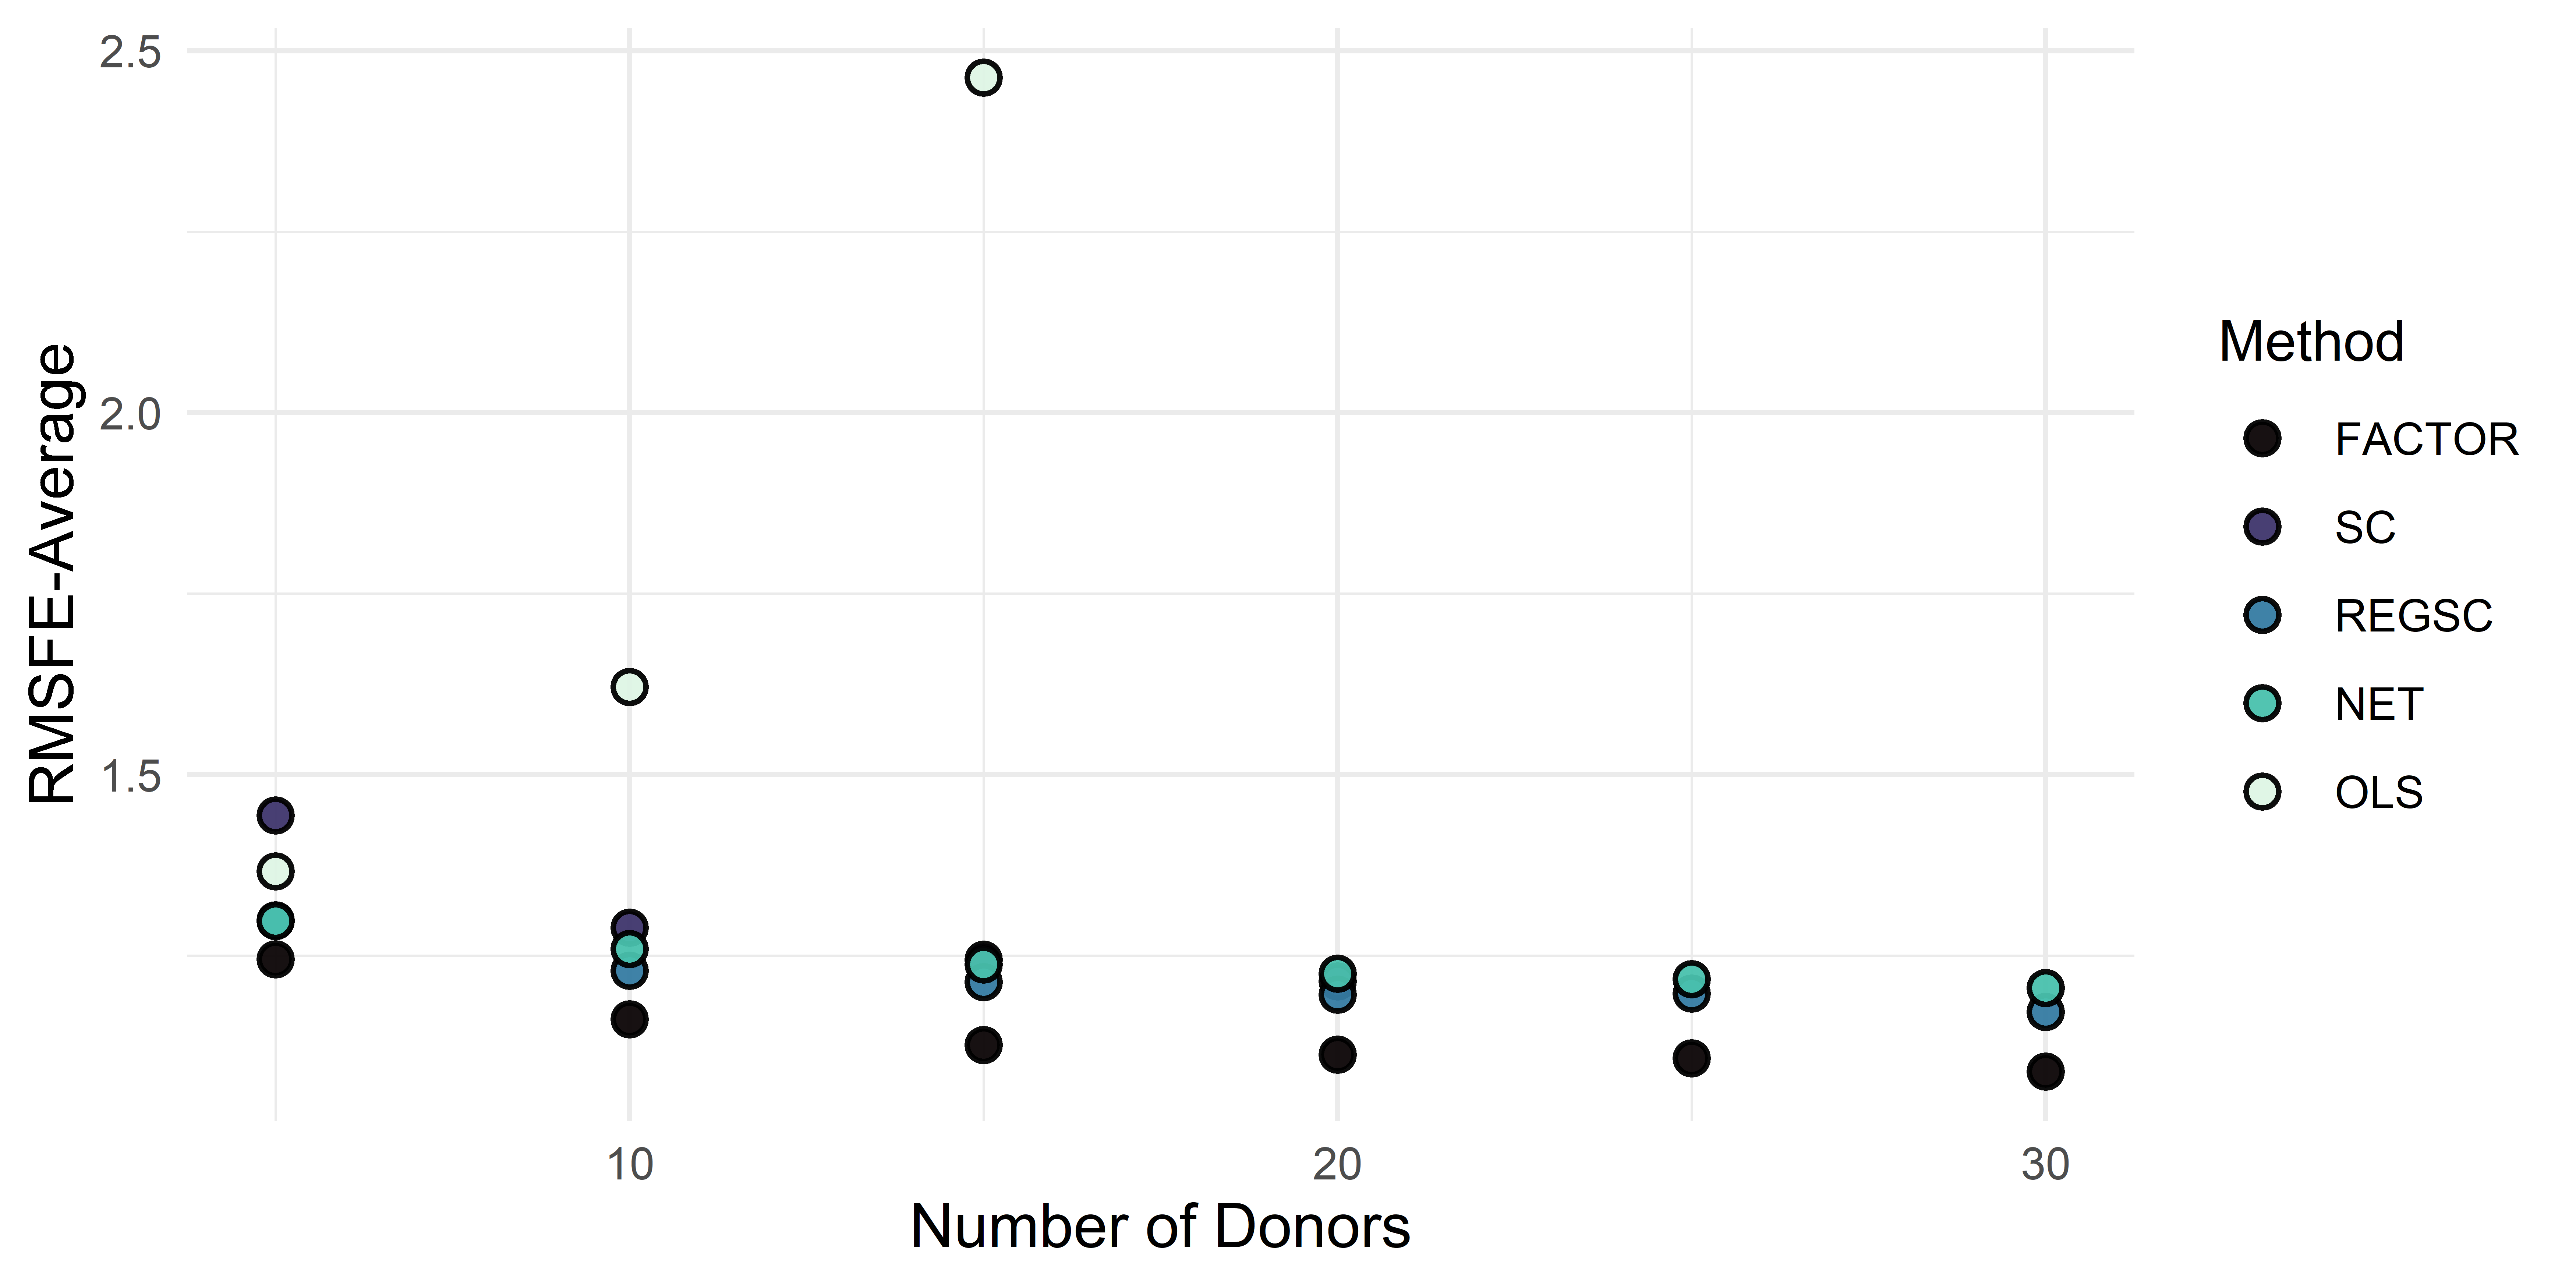
\includegraphics[scale=.9]{F06}
	\caption{Simulation Performance for $T_{pre} = 20$ and $T_{post} \in \left\lbrace 10,20,30\right\rbrace$}
	\label{F_10}
\end{figure}

\begin{figure}[H]
	\centering
	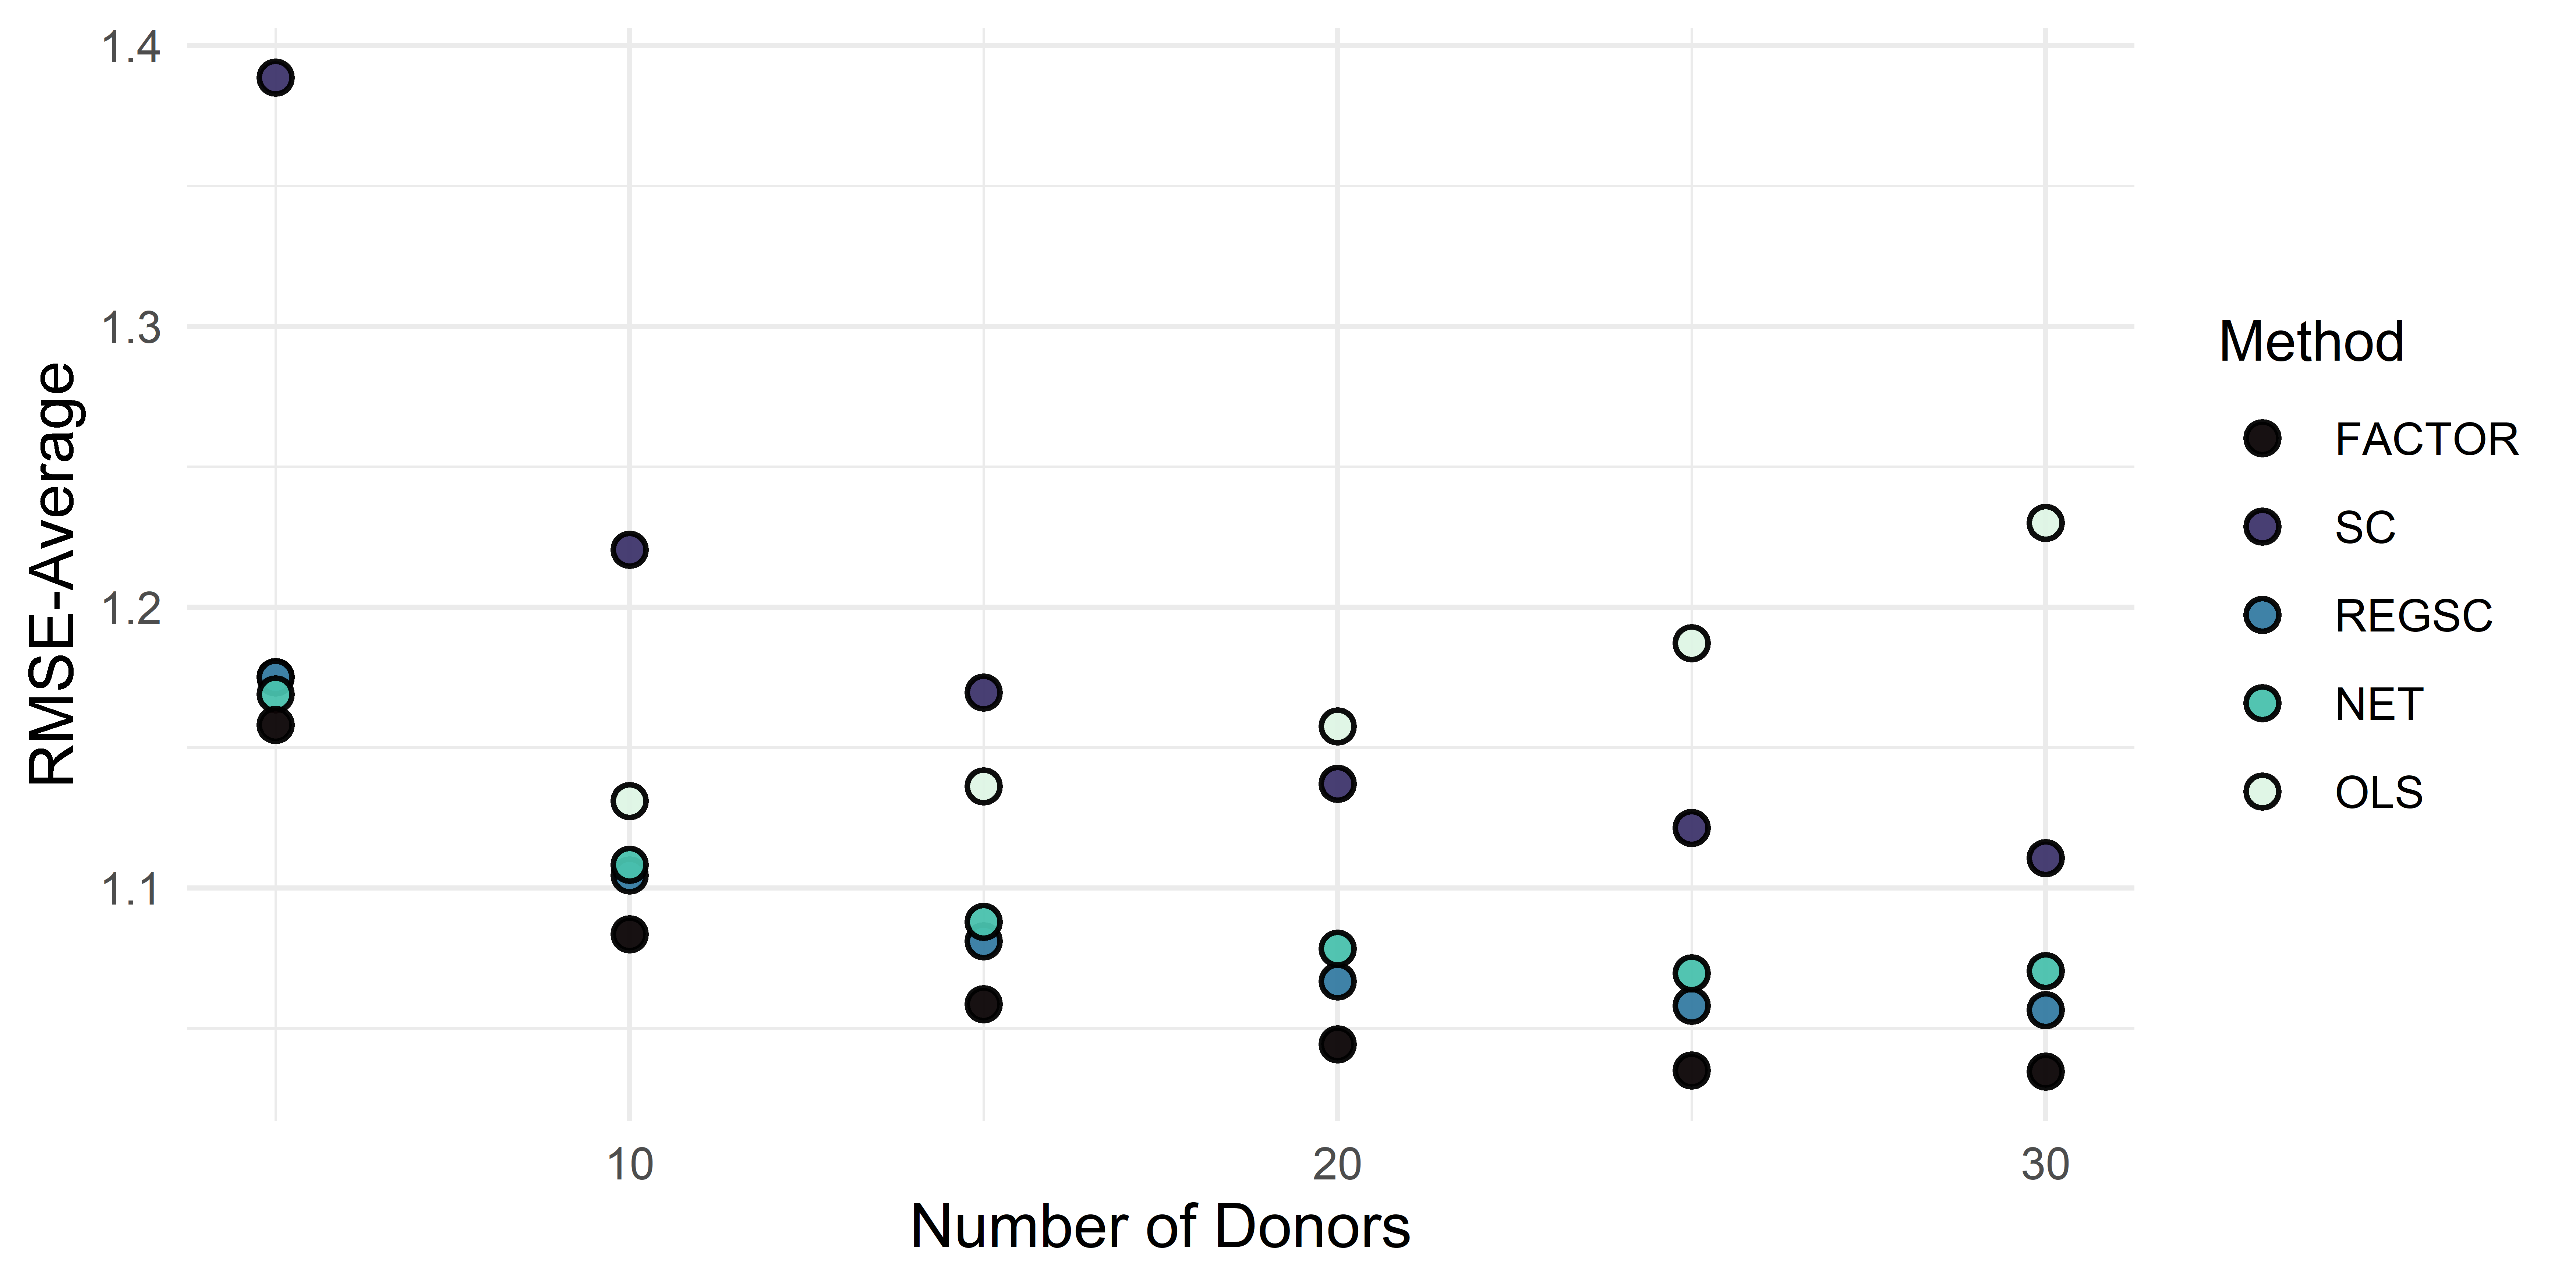
\includegraphics[scale=.9]{F08}
	\caption{Simulation Performance for $T_{pre} = 100$ and $T_{post} \in \left\lbrace 10,20,30\right\rbrace$}
	\label{F_11}
\end{figure}

\newpage
\begin{figure}[H]
	\centering
	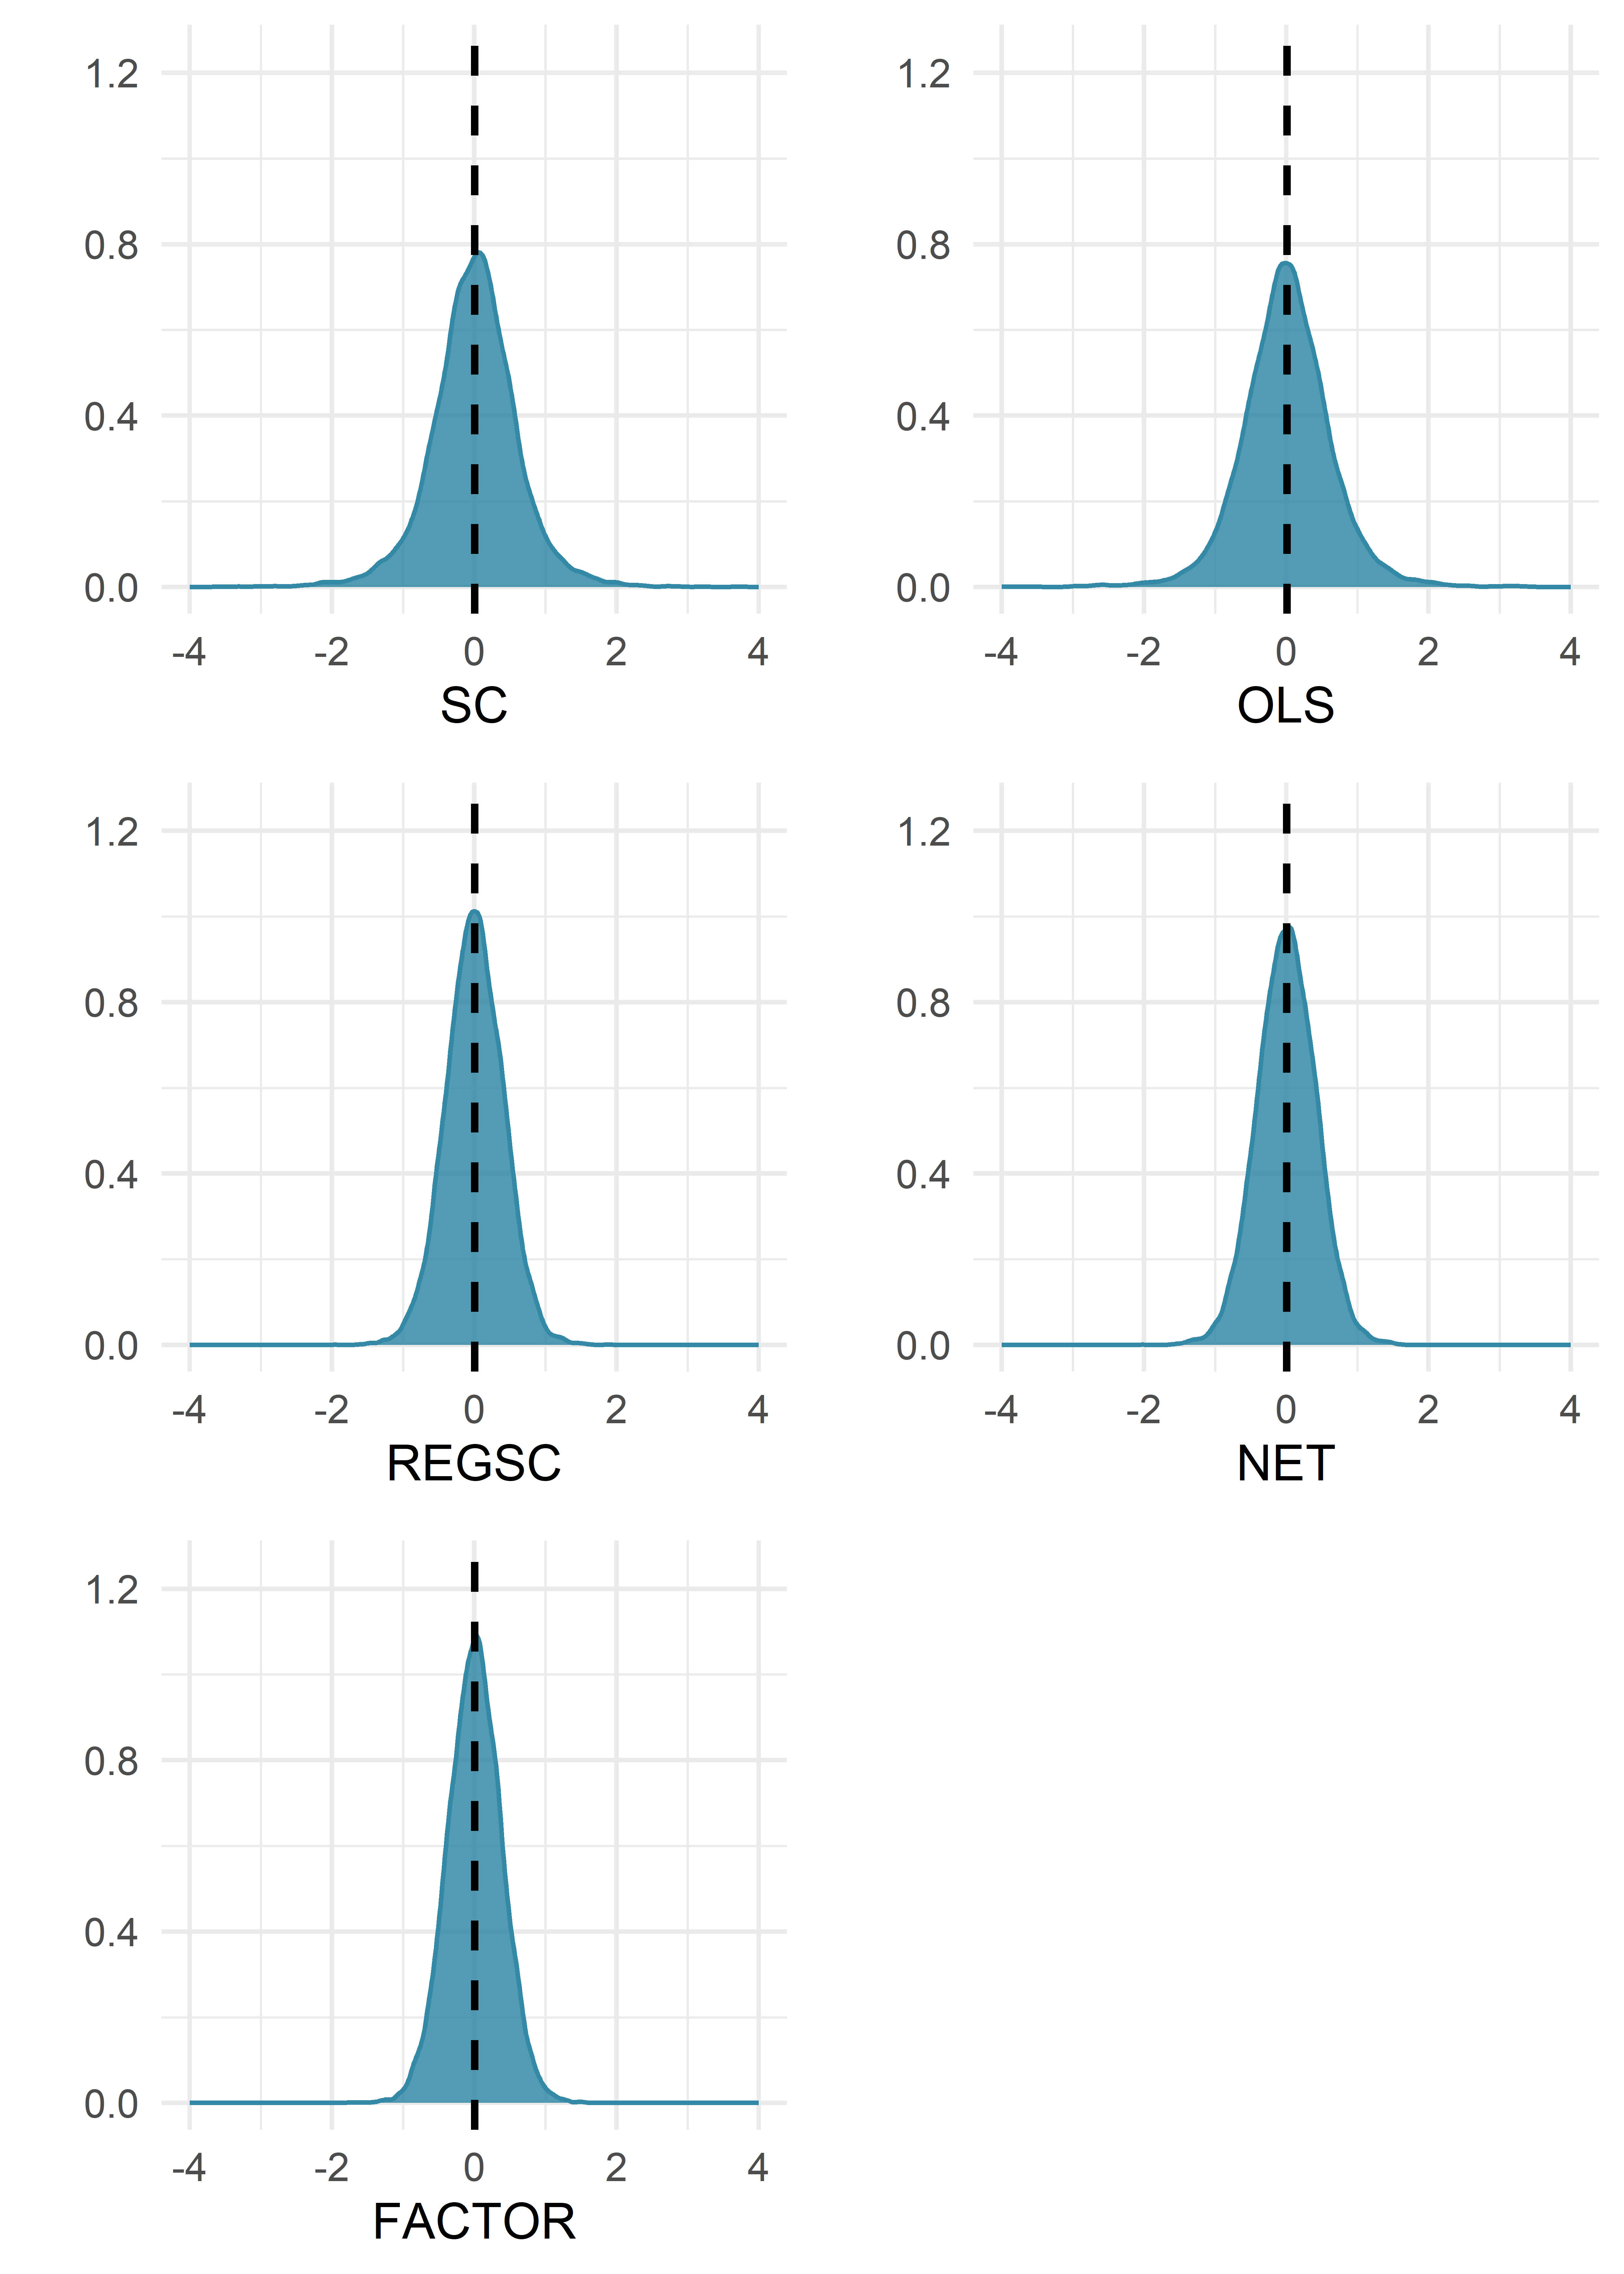
\includegraphics[scale=.9]{F17}
	\caption{Bias-densities for $T_{pre} = 20$ and $T_{post} \in \left\lbrace 10,20,30\right\rbrace$}
	\label{F_12}
\end{figure}

\newpage
\begin{figure}[H]
	\centering
	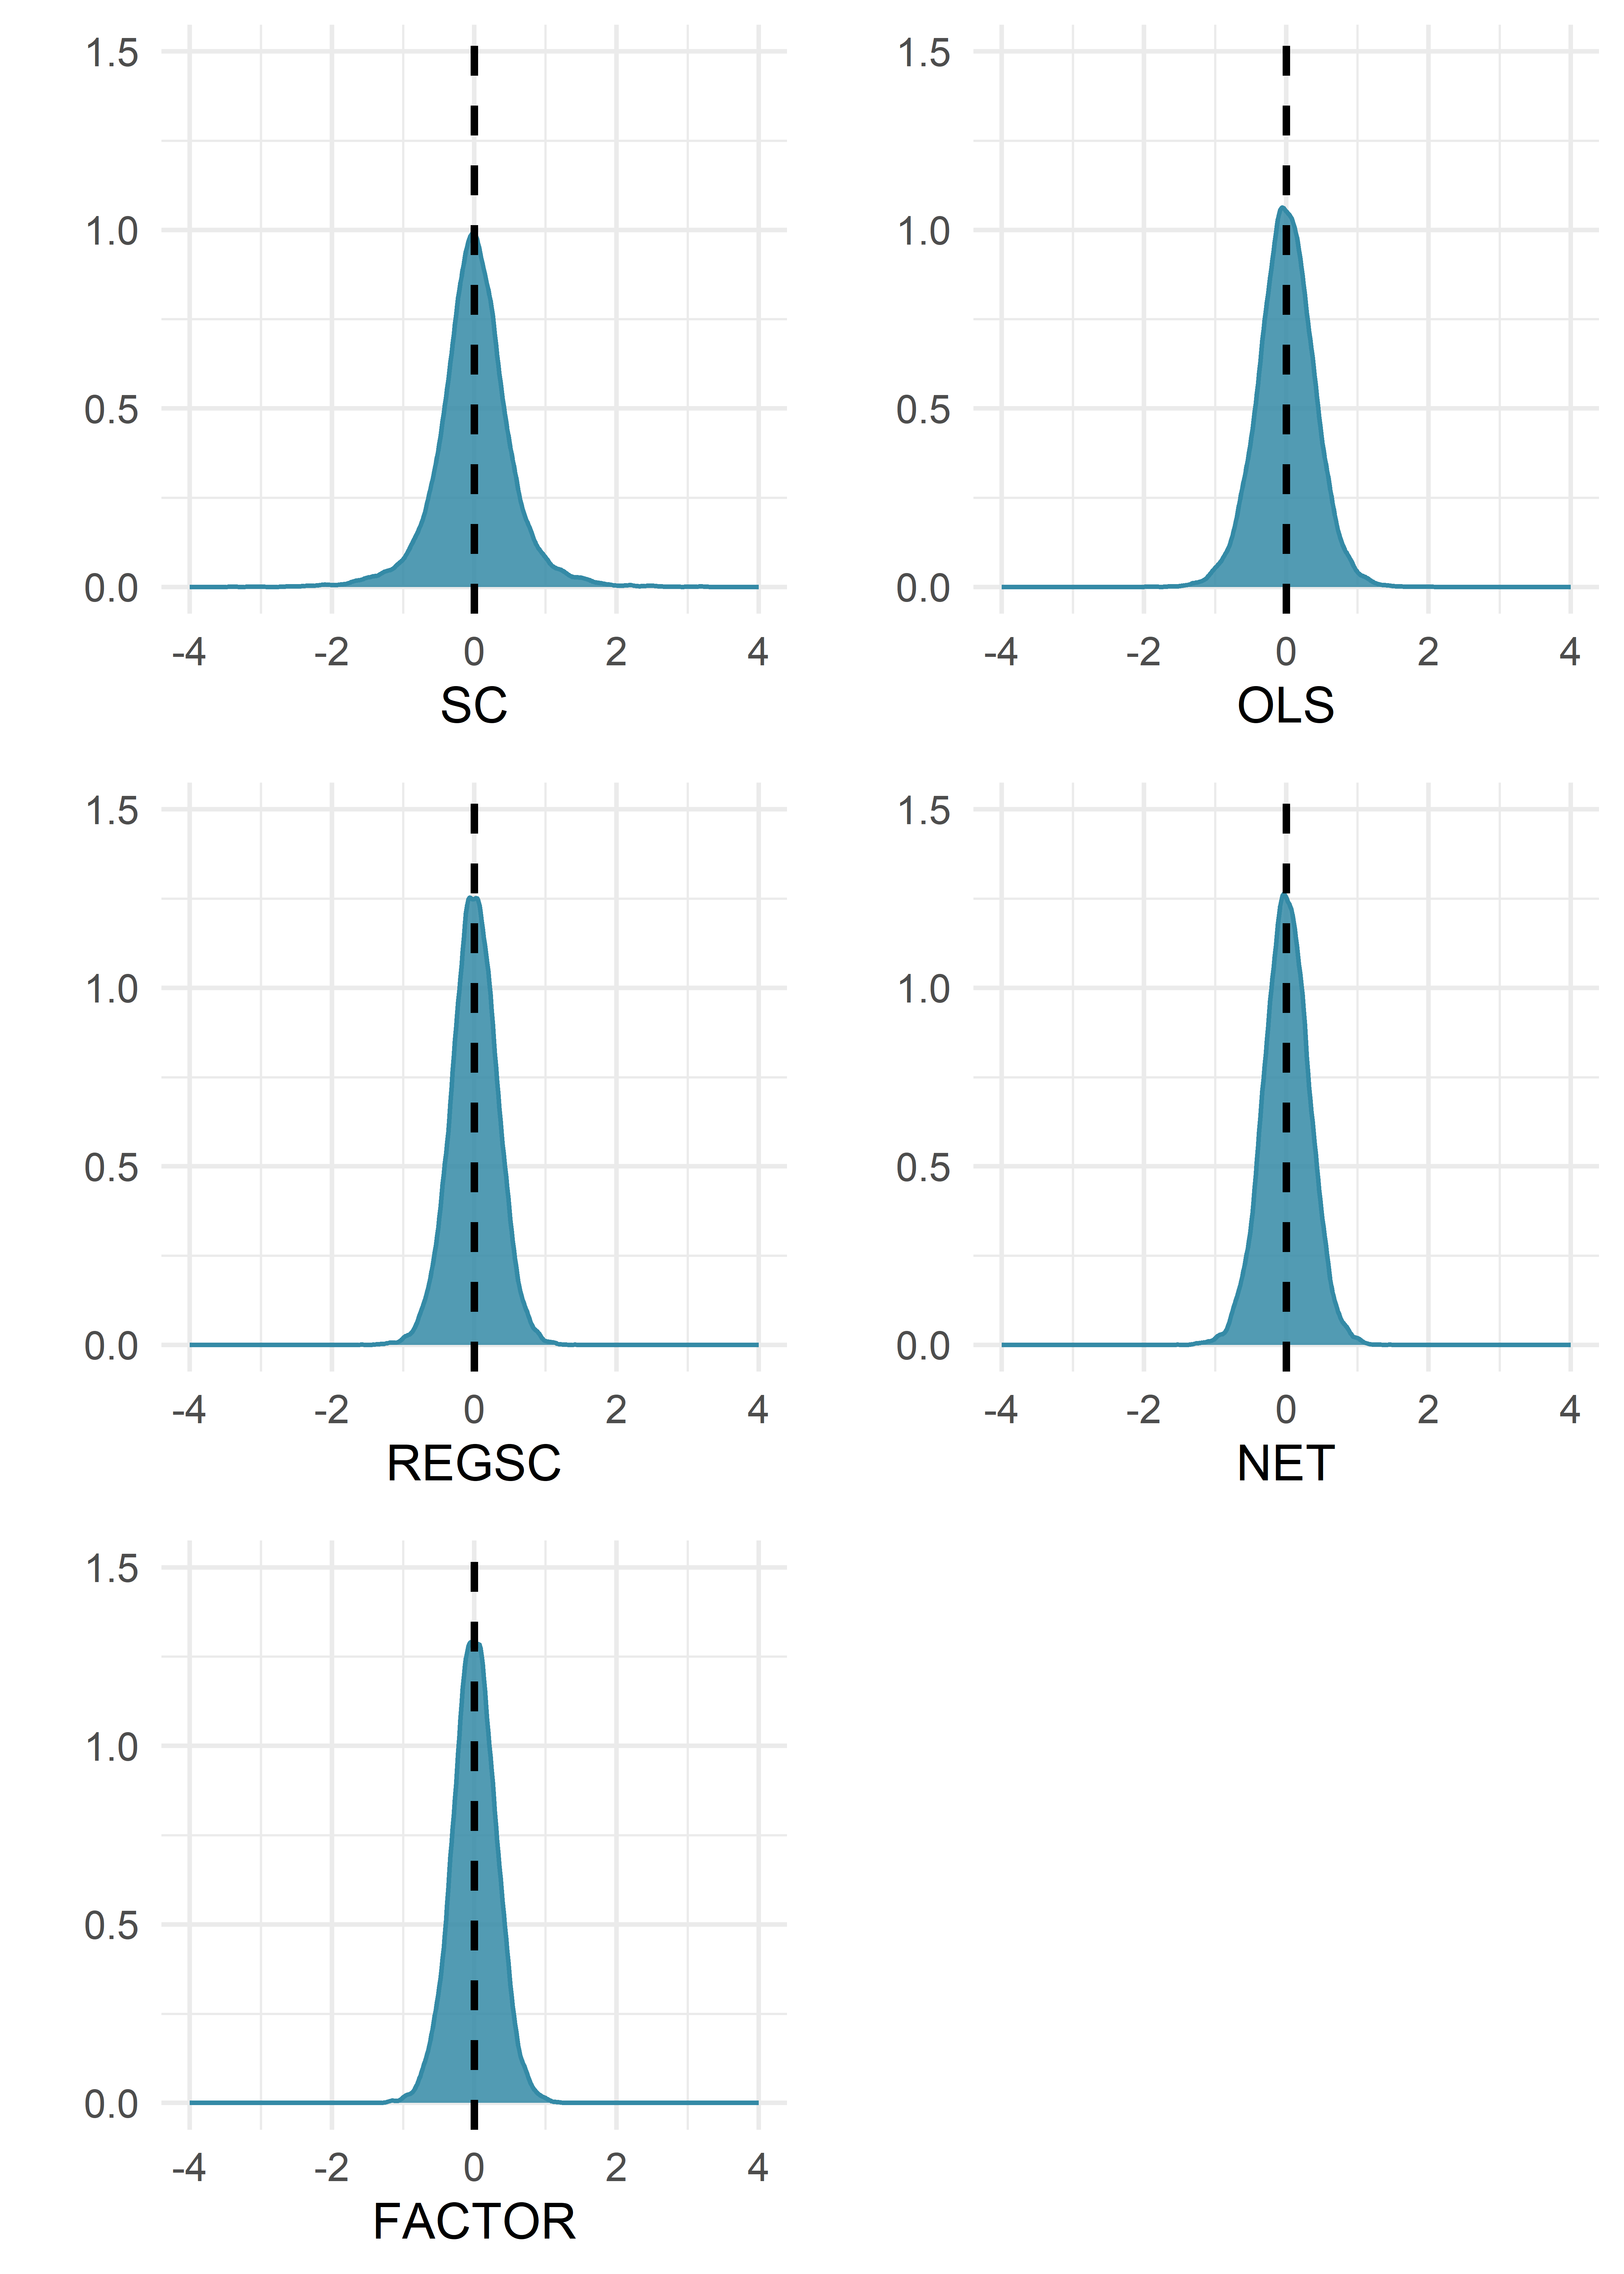
\includegraphics[scale=.9]{F18}
	\caption{Bias-densities for $T_{pre} = 50$ and $T_{post} \in \left\lbrace 10,20,30\right\rbrace$}
	\label{F_13}
\end{figure}

\newpage
\begin{figure}[H]
	\centering
	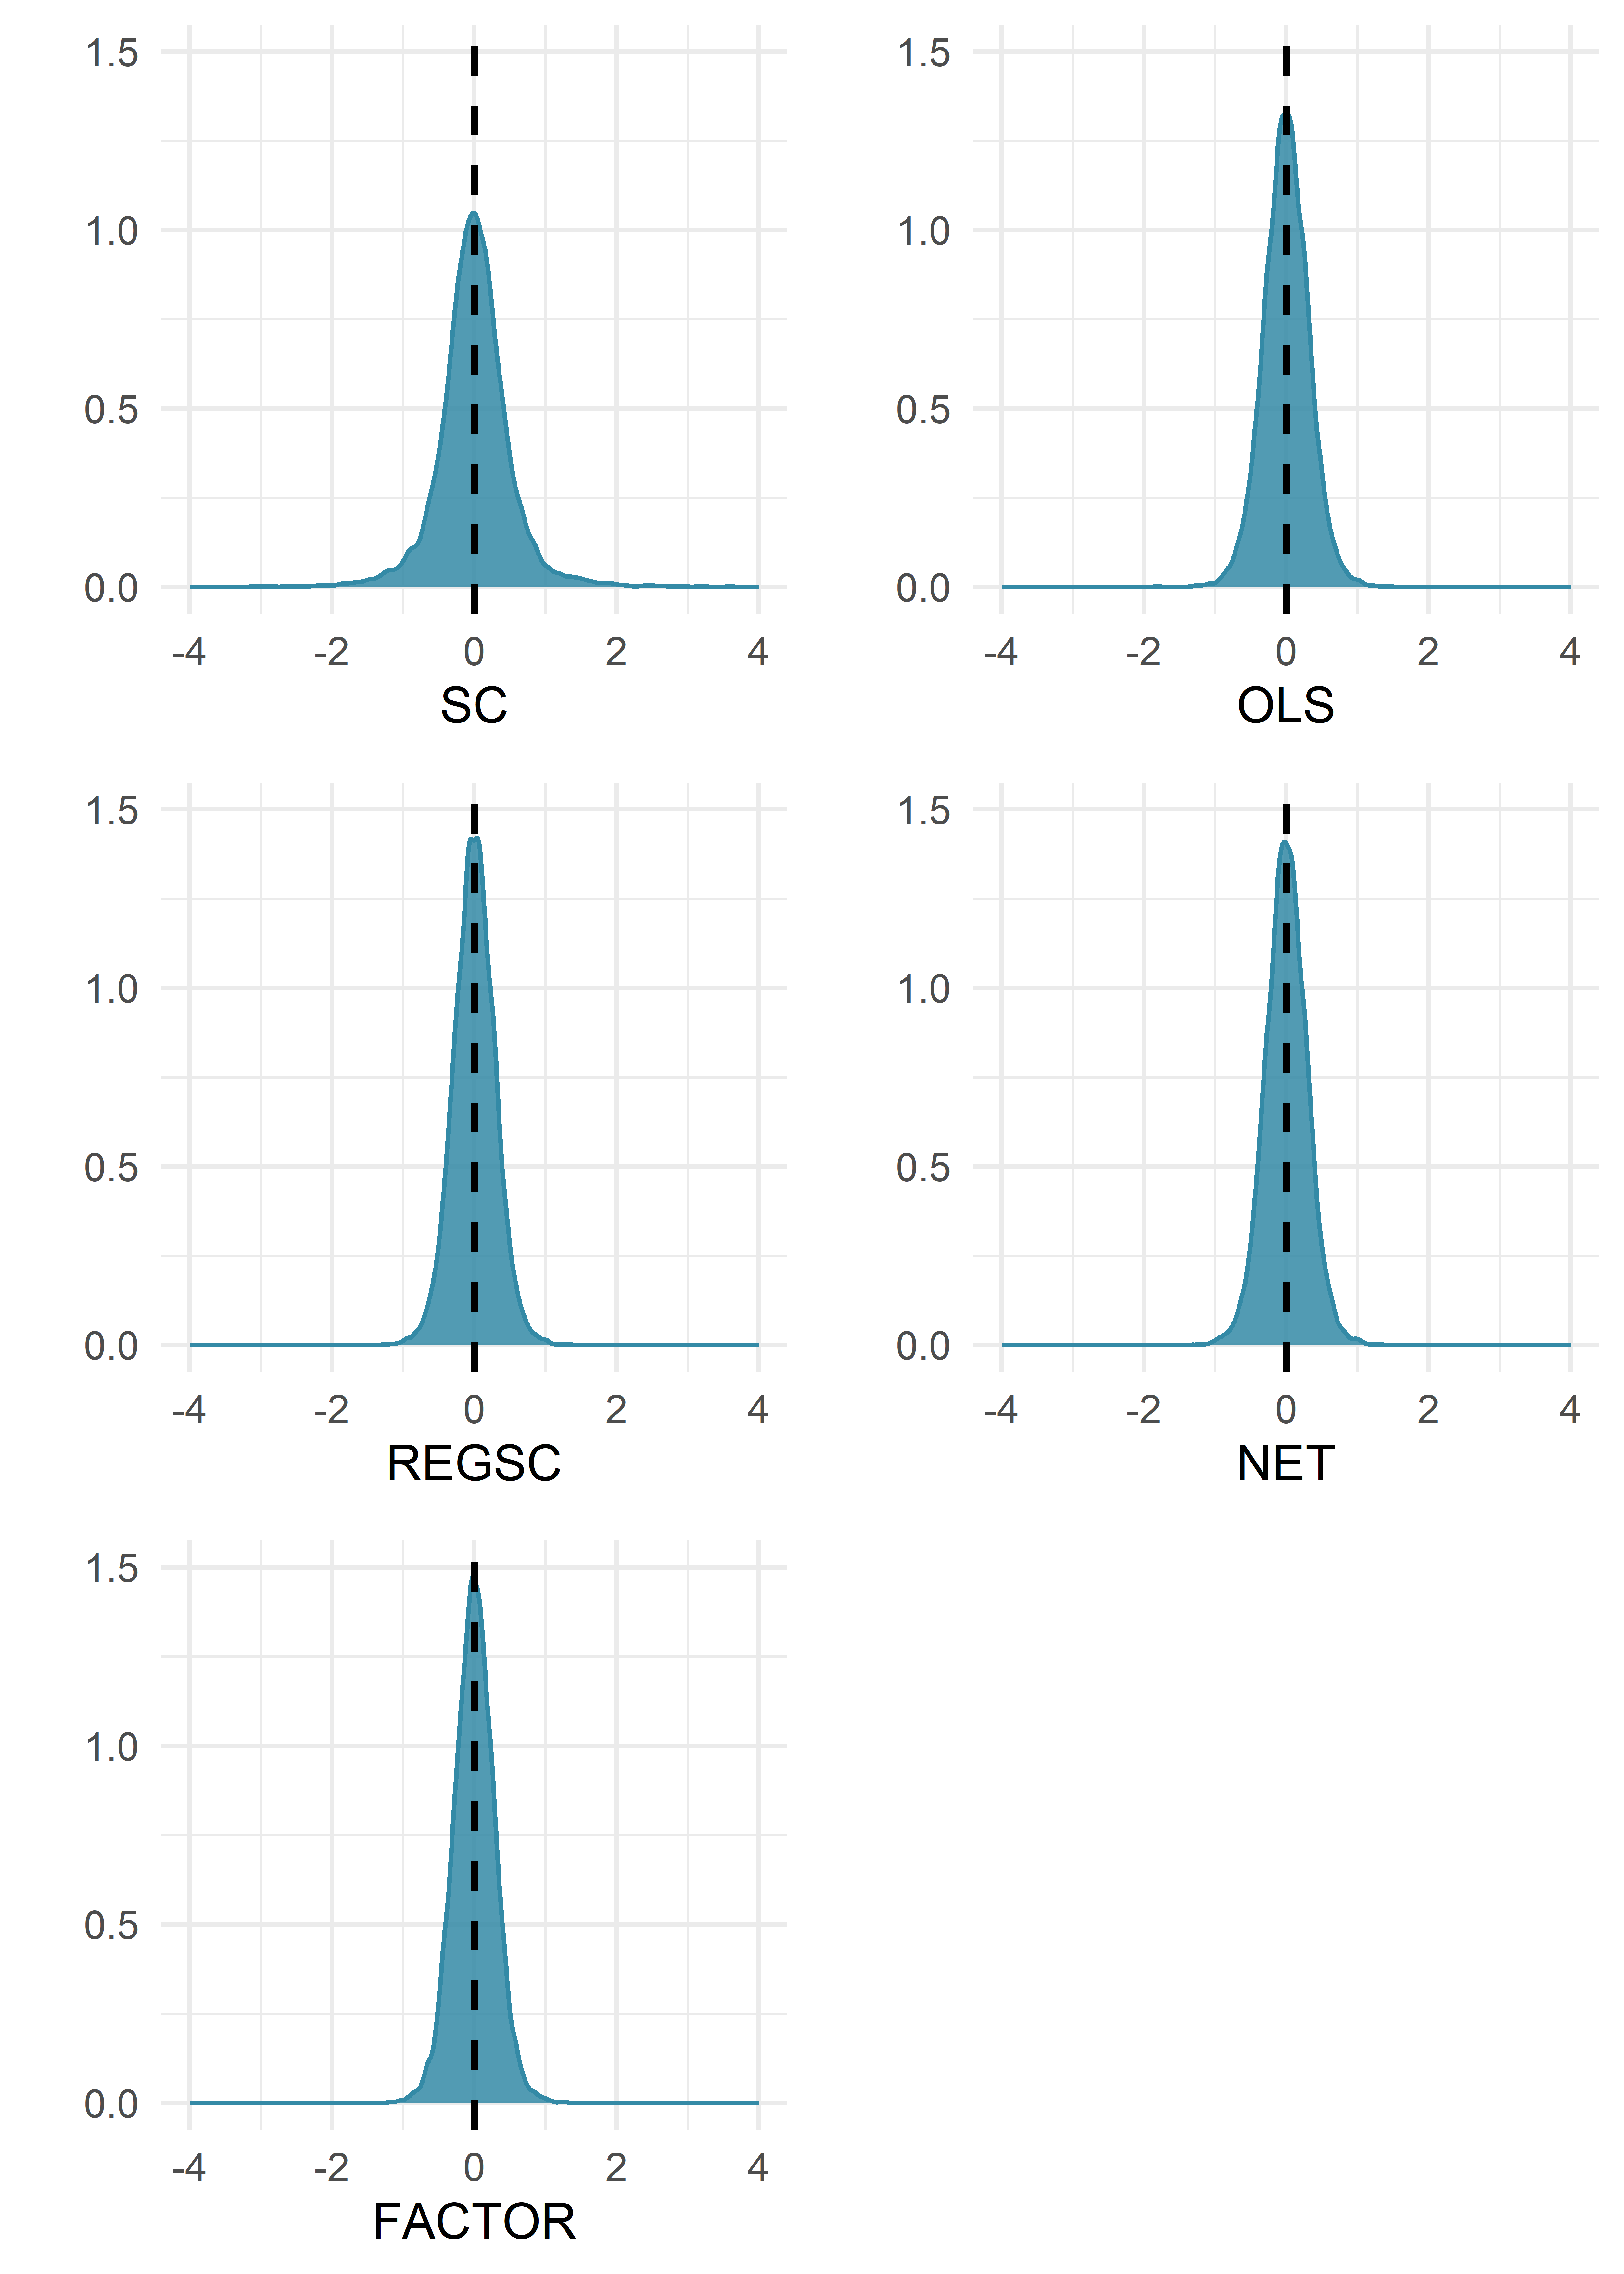
\includegraphics[scale=.9]{F19}
	\caption{Bias-densities for $T_{pre} = 100$ and $T_{post} \in \left\lbrace 10,20,30\right\rbrace$}
	\label{F_14}
\end{figure}

\newpage
\begin{table}[H]
	\centering
	\noindent
	\caption{RMSFE results for $T_{pre} = \in \left\lbrace 20,50,100\right\rbrace$ and $J \in \left\lbrace 5,10,15,20,25,30\right\rbrace$}
	\scalebox{1}{
		\begin{tabular}{c c | C{1.5cm} | C{1.5cm} | C{1.5cm} | C{1.5cm} | C{1.5cm} | C{1.5cm} }
			\toprule[1.5pt]
			\multicolumn{1}{c}{$\boldsymbol{T_{pre}}$} & \multicolumn{1}{c}{\textbf{Donors}}& \multicolumn{1}{c}{\textbf{SC}} & \multicolumn{1}{c}{\textbf{OLS}} & \multicolumn{1}{c}{\textbf{REGSC}}& \multicolumn{1}{c}{\textbf{NET}}& \multicolumn{1}{c}{\textbf{FACTOR}} & \multicolumn{1}{c}{\textbf{2nd best}}\\
			\cmidrule(lr){1-8}
			20&5&1.4438&1.3665&1.2988&1.2980&1.2450&NET\\
			20&10&1.2889&1.6212&1.2294&1.2591&1.1620&REGSC\\
			20&15&1.2444&2.4629&1.2133&1.2377&1.1266&REGSC\\
			20&20&1.2144&NA&1.1961&1.2251&1.1132&REGSC\\
			20&25&NA&NA&1.1976&1.2175&1.1081&REGSC\\
			20&30&NA&NA&1.1724&1.2051&1.0901&REGSC\\
			\cmidrule(lr){1-8}
			50&5&1.4126&1.2101&1.2038&1.1946&1.1735&NET\\
			50&10&1.2366&1.2006&1.1318&1.1404&1.0957&REGSC\\
			50&15&1.1888&1.2640&1.1134&1.1276&1.0740&REGSC\\
			50&20&1.1649&1.3491&1.0999&1.1157&1.0643&REGSC\\
			50&25&1.1515&1.4856&1.0952&1.1104&1.0570&REGSC\\
			50&30&1.1377&1.6422&1.0867&1.1074&1.0474&REGSC\\
			\cmidrule(lr){1-8}
			100&5&1.3886&1.1750&1.1750&1.1689&1.1580&NET\\
			100&10&1.2205&1.1308&1.1044&1.1082&1.0835&REGSC\\
			100&15&1.1695&1.1361&1.0810&1.0879&1.0585&REGSC\\
			100&20&1.1371&1.1575&1.0667&1.0783&1.0443&REGSC\\
			100&25&1.1213&1.1871&1.0580&1.0695&1.0349&REGSC\\
			100&30&1.1105&1.2299&1.0565&1.0704&1.0346&REGSC\\
			\bottomrule[1.5pt]
	\end{tabular}}
	\label{table:table S.8}
\end{table}